% Preamble templated from Mihir-Divyansh/Course-Setup
%iffalse
\let\negmedspace\undefined
\let\negthickspace\undefined
\documentclass[journal,12pt,onecolumn]{IEEEtran}
\usepackage{cite}
\usepackage{amsmath,amssymb,amsfonts,amsthm}
\usepackage{algorithmic}
\usepackage{graphicx}
\usepackage{textcomp}
\usepackage{xcolor}
\usepackage{txfonts}
\usepackage{listings}
\usepackage{enumitem}
\usepackage{mathtools}
\usepackage{gensymb}
\usepackage{comment}
\usepackage[breaklinks=true]{hyperref}
\usepackage{tkz-euclide}
\usepackage{listings}
\usepackage{gvv}
%\def\inputGnumericTable{}
\usepackage[latin1]{inputenc}
\usepackage{color}
\usepackage{array}
\usepackage{longtable}
\usepackage{calc}
\usepackage{multirow}
\usepackage{hhline}
\usepackage{ifthen}
\usepackage{lscape}
\usepackage{tabularx}
\usepackage{array}
\usepackage{float}
\usepackage{caption}
\usepackage{multicol}

\newtheorem{theorem}{Theorem}[section]
\newtheorem{problem}{Problem}
\newtheorem{proposition}{Proposition}[section]
\newtheorem{lemma}{Lemma}[section]
\newtheorem{corollary}[theorem]{Corollary}
\newtheorem{example}{Example}[section]
\newtheorem{definition}[problem]{Definition}
\newcommand{\BEQA}{\begin{eqnarray}}
\newcommand{\EEQA}{\end{eqnarray}}
\newcommand{\define}{\stackrel{\triangle}{=}}
\theoremstyle{remark}
\newtheorem{rem}{Remark}

% Marks the beginning of the document
\begin{document}
\bibliographystyle{IEEEtran}
\vspace{3cm}

\title{Assignment 1: GATE 2010 PH: Physics}
\author{EE25BTECH11055 - Subhodeep Chakraborty}
\maketitle
\hrulefill
\bigskip

\renewcommand{\thefigure}{\theenumi}
\renewcommand{\thetable}{\theenumi}


\begin{enumerate}
\item Consider an anti-symmetric tensor $P_{U}$ with the indices i and j running from 1 to 5. The number of independent components of the tensor is \hfill\brak{\text{GATE PH 2010}}


\begin{enumerate} \begin{multicols}{4}
	\item 3 \item 10 \item 9 \item 6
\end{multicols} \end{enumerate}

\item The value of the integral $\oint\limits_{C}\frac{e^{z}\sin(z)}{z^{2}}dz$ where the contour C is the unit circle: $|z-2|=1$, is\hfill\brak{\text{GATE PH 2010}}


\begin{enumerate} \begin{multicols}{4}
	\item 2$\pi i$ \item 4$\pi i$ \item $\pi i$ \item 0
\end{multicols} \end{enumerate}

\item The eigenvalues of the matrix $\myvec{ 2 & 3 & 0 \\ 3 & 2 & 0 \\ 0 & 0 & 1 }$ are\hfill\brak{\text{GATE PH 2010}}


\begin{enumerate} \begin{multicols}{4}
	\item 5, 2, -2 \item -5, -1, -1 \item 5, 1, -1 \item -5, 1, 1
\end{multicols} \end{enumerate}

\item If $f(x)=\begin{cases}0& \text{for } x<3, \\ x-3& \text{for } x\ge3, \end{cases}$ then the Laplace transform of $f(x)$ is\hfill\brak{\text{GATE PH 2010}}

\begin{enumerate} \begin{multicols}{4}
	\item $s^{-2}e^{3s}$ \item $s^{2}e^{-3s}$ \item $s^{-2}$ \item $s^{-2}e^{-3s}$
\end{multicols} \end{enumerate}

\item The valence electrons do not directly determine the following property of a metal.\hfill\brak{\text{GATE PH 2010}}

\begin{enumerate}
\begin{multicols}{2}
\item Electrical conductivity
\item Thermal conductivity
\item Shear modulus
\item Metallic lustre
\end{multicols}
\end{enumerate}

\item Consider X-ray diffraction from a crystal with a face-centered-cubic (fcc) lattice. The lattice plane for which there is NO diffraction peak is\hfill\brak{\text{GATE PH 2010}}

\begin{enumerate} \begin{multicols}{4}
	\item (2, 1, 2) \item (1, 1, 1) \item (2, 0, 0) \item (3, 1, 1)
\end{multicols} \end{enumerate}

\item The Hall coefficient, $R_H$, of sodium depends on\hfill\brak{\text{GATE PH 2010}}

\begin{enumerate}
\item The effective charge carrier mass and carrier density
\item The charge carrier density and relaxation time
\item The charge carrier density only
\item The effective charge carrier mass
\end{enumerate}

\item The Bloch theorem states that within a crystal, the wavefunction, $\psi(\vec{r})$, of an electron has the form\hfill\brak{\text{GATE PH 2010}}

\begin{enumerate}
	\item $\psi(\vec{r})=u(\vec{r})e^{i\vec{k}\cdot\vec{r}}$ where $u(\vec{r})$ is an arbitrary function and $\vec{k}$ is an arbitrary vector
	\item $\psi(\vec{r})=u(\vec{r})e^{i\vec{G}\cdot\vec{r}}$ where $u(\vec{r})$ is an arbitrary function and $\vec{G}$ is a reciprocal lattice vector
	\item $\psi(\vec{r})=u(\vec{r})e^{i\vec{G}\cdot\vec{r}}$ where $u(\vec{r})=u(\vec{r}+\vec{\Lambda})$, $\vec{\Lambda}$ is a lattice vector and $\vec{G}$ is a reciprocal lattice vector
	\item $\psi(\vec{r})=u(\vec{r})e^{i\vec{k}\cdot\vec{r}}$ where $u(\vec{r})=u(\vec{r}+\vec{\Lambda})$, $\vec{\Lambda}$ is a lattice vector and $\vec{k}$ is an arbitrary vector
\end{enumerate}

\item In an experiment involving a ferromagnetic medium, the following observations were made. Which one of the plots does NOT correctly represent the property of the medium? ($T_C$ is the Curie temperature)\hfill\brak{\text{GATE PH 2010}}
\begin{figure}[H]
\begin{multicols}{2}
	\centering
	\caption*{} \label{fig:9a} 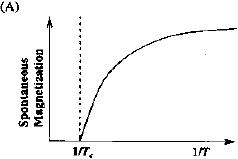
\includegraphics[width=0.45\columnwidth]{figs/9a.png}
	\caption*{} \label{fig:9b} 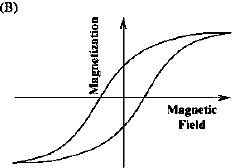
\includegraphics[width=0.45\columnwidth]{figs/9b.png}
	\caption*{} \label{fig:9c} 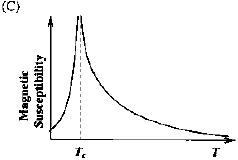
\includegraphics[width=0.45\columnwidth]{figs/9c.png}
	\caption*{} \label{fig:9d} 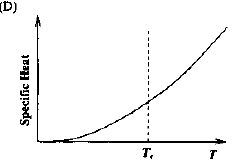
\includegraphics[width=0.45\columnwidth]{figs/9d.png}
	\end{multicols}
\end{figure}

\item The thermal conductivity of a given material reduces when it undergoes a transition from its normal state to the superconducting state. The reason is:\hfill\brak{\text{GATE PH 2010}}

\begin{enumerate}
	\item The Cooper pairs cannot transfer energy to the lattice
	\item Upon the formation of Cooper pairs, the lattice becomes less efficient in heat transfer
	\item The electrons in the normal state lose their ability to transfer heat because of their coupling to the Cooper pairs
	\item The heat capacity increases on transition to the superconducting state leading to a reduction in thermal conductivity
\end{enumerate}

\item The basic process underlying the neutron $\beta$-decay is\hfill\brak{\text{GATE PH 2010}}

\begin{enumerate} \begin{multicols}{4}
	\item $d \rightarrow u + e^{-} + \overline{v}_{e}$
	\item $d \rightarrow u + e^{-}$
	\item $s \rightarrow u + e^{-} + \overline{v}_{e}$
	\item $u \rightarrow d + e^{+} + \overline{v}_{e}$
\end{multicols} \end{enumerate}

\item In the nuclear shell model the spin parity of ${}^{15}N$ is given by\hfill\brak{\text{GATE PH 2010}}

\begin{enumerate} \begin{multicols}{4}
	\item $\frac{1}{2}^{-}$ \item $\frac{1}{2}^{+}$ \item $\frac{3}{2}^{-}$ \item $\frac{3}{2}^{+}$
\end{multicols} \end{enumerate}

\item Match the reactions on the left with the associated interactions on the right.\hfill\brak{\text{GATE PH 2010}}

\begin{multicols}{2}
\begin{enumerate}%[label=(\arabic*)]
		\item $\pi^{+} \rightarrow \mu^{+} + \nu_{\mu}$
		\item $\pi^{0} \rightarrow \gamma + \gamma$
		\item $\pi^{0} + n \rightarrow \pi^{-} + p$
	\end{enumerate}
\columnbreak
\begin{enumerate}%[label=(\roman*)]
		\item Strong
		\item Electromagnetic
		\item Weak
	\end{enumerate}
\end{multicols}

\begin{enumerate} \begin{multicols}{4}
	\item \brak{\text{a, c}}, \brak{\text{b, b}}, \brak{\text{c, a}} \item \brak{\text{a, a}}, \brak{\text{b, b}}, \brak{\text{c, c}}
	\item \brak{\text{a, b}}, \brak{\text{b, a}}, \brak{\text{c, c}} \item \brak{\text{a, c}}, \brak{\text{b, a}}, \brak{\text{c, b}}
\end{multicols} \end{enumerate}

\item To detect trace amounts of a gaseous species in a mixture of gases, the preferred probing tool is\hfill\brak{\text{GATE PH 2010}}

\begin{enumerate}
	\begin{multicols}{2}
\item Ionization spectroscopy with X-rays \item NMR spectroscopy
	\item ESR spectroscopy \item Laser spectroscopy
	\end{multicols}
\end{enumerate}

\item A collection of N atoms is exposed to a strong resonant electromagnetic radiation with $N_g$ atoms in the ground state and $N_e$ atoms in the excited state, such that $N_g+N_e=N$. This collection of two-level atoms will have the following population distribution:\hfill\brak{\text{GATE PH 2010}}

\begin{enumerate} \begin{multicols}{4}
	\item $N_g \ll N_e$ \item $N_g \gg N_e$ \item $N_g \approx N_e = N/2$ \item $N_g - N_e \approx N/2$
\end{multicols} \end{enumerate}

\item Two states of an atom have definite parities. An electric dipole transition between these states is\hfill\brak{\text{GATE PH 2010}}

\begin{enumerate}
	\item Allowed if both the states have even parity
	\item Allowed if both the states have odd parity
	\item Allowed if the two states have opposite parities
	\item Not allowed unless a static electric field is applied
\end{enumerate}

\item The spectrum of radiation emitted by a black body at a temperature 1000 K peaks in the\hfill\brak{\text{GATE PH 2010}}

\begin{enumerate}
	\begin{multicols}{2}
	 \item Visible range of frequencies \item Infrared range of frequencies
	\item Ultraviolet range of frequencies \item Microwave range of frequencies
	\end{multicols}
\end{enumerate}

\item An insulating sphere of radius a carries a charge density $\rho(\vec{r})=\rho_{0}(a^{2}-r^{2})\cos\theta; r<a$. The leading order term for the electric field at a distance d, far away from the charge distribution, is proportional to\hfill\brak{\text{GATE PH 2010}}

\begin{enumerate} \begin{multicols}{4}
	\item $d^{-1}$ \item $d^{-2}$ \item $d^{-3}$ \item $d^{-4}$
\end{multicols} \end{enumerate}

\item The voltage resolution of a 12-bit digital to analog converter (DAC), whose output varies from -10 V to +10 V is, approximately\hfill\brak{\text{GATE PH 2010}}

\begin{enumerate} \begin{multicols}{4}
	\item 1 mV \item 5 mV \item 20 mV \item 100 mV
\end{multicols} \end{enumerate}

\item In one of the following circuits, negative feedback does not operate for a negative input. Which one is it? The opamps are running from $\pm$15 V supplies.\hfill\brak{\text{GATE PH 2010}}
\begin{figure}[H]
	\centering
	\caption*{} \label{fig:20} 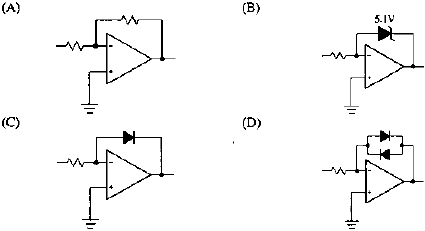
\includegraphics[width=0.9\columnwidth]{figs/20.png}
\end{figure}

\item A system of N non-interacting classical point particles is constrained to move on the two-dimensional surface of a sphere. The internal energy of the system is\hfill\brak{\text{GATE PH 2010}}

\begin{enumerate} \begin{multicols}{4}
	\item $\frac{3}{2}Nk_{B}T$ \item $\frac{1}{2}Nk_{B}T$ \item $Nk_{B}T$ \item $\frac{5}{2}Nk_{B}T$
\end{multicols} \end{enumerate}

\item Which of the following atoms cannot exhibit Bose-Einstein condensation, even in principle?\hfill\brak{\text{GATE PH 2010}}

\begin{enumerate} \begin{multicols}{4}
	\item $^{1}H_{1}$ \item $^{4}He_{2}$ \item $^{23}Na_{11}$ \item $^{40}K_{19}$
\end{multicols} \end{enumerate}

\item For the set of all Lorentz transformations with velocities along the x-axis, consider the two statements given below:
	\begin{itemize}
		\item[P:] If L is a Lorentz transformation then, $L^{-1}$ is also a Lorentz transformation.
		\item[Q:] If $L_1$ and $L_2$ are Lorentz transformations then, $L_1L_2$ is necessarily a Lorentz transformation.
	\end{itemize}
	Choose the correct option.\hfill\brak{\text{GATE PH 2010}}

\begin{enumerate}
\begin{multicols}{2}
	\item P is true and Q is false. \item Both P and Q are true.
	\item Both P and Q are false. \item P is false and Q is true.
	\end{multicols}
\end{enumerate}

\item Which of the following is an allowed wavefunction for a particle in a bound state? N is a constant and $\alpha, \beta > 0$.\hfill\brak{\text{GATE PH 2010}}

\begin{enumerate}
	\begin{multicols}{2}
	 \item $\psi=N\frac{e^{-\alpha r}}{r^{3}}$
	\item $\psi=N(1-e^{-\alpha r})$
	\item $\psi=Ne^{-\alpha x}e^{-\beta(x^{2}+y^{2}+z^{2})}$
	\item $\psi=\begin{cases} \text{non-zero constant} & \text{if } r<R \\ 0 & \text{if } r>R \end{cases}$
	\end{multicols}
\end{enumerate}

\item A particle is confined within a spherical region of radius one femtometer ($10^{-15}$m). Its momentum can be expected to be about\hfill\brak{\text{GATE PH 2010}}

\begin{enumerate} \begin{multicols}{4}
	\item $20 \frac{\text{keV}}{c}$ \item $200 \frac{\text{keV}}{c}$ \item $200 \frac{\text{MeV}}{c}$ \item $2 \frac{\text{GeV}}{c}$
\end{multicols} \end{enumerate}


\item For the complex function, $f(z)=\frac{e^{\sqrt{z}}-e^{-\sqrt{z}}}{\sin(\sqrt{z})},$ which of the following statements is correct?\hfill\brak{\text{GATE PH 2010}}

\begin{enumerate}
	\item $z=0$ is a branch point \item $z=0$ is a pole of order one
	\item $z=0$ is a removable singularity \item $z=0$ is an essential singularity
\end{enumerate}

\item The solution of the differential equation for $y(t): \frac{d^{2}y}{dt^{2}}-y=2\cosh(t)$, subject to the initial conditions $y(0)=0$ and $\frac{dy}{dt}|_{t=0}=0,$ is\hfill\brak{\text{GATE PH 2010}}

\begin{enumerate}
	\begin{multicols}{2}
	 \item $\frac{1}{2}\cosh(t)+t\sinh(t)$ \item $-\sinh(t)+t\cosh(t)$
	\item $t\cosh(t)$ \item $t\sinh(t)$
	\end{multicols}
\end{enumerate}

\item Given the recurrence relation for the Legendre polynomials
\begin{align*}(2n+1) x P_n(x)=(n+1) P_{n+1}(x)+nP_{n-1}(x),
\end{align*}
which of the following integrals has a non-zero value?\hfill\brak{\text{GATE PH 2010}}

\begin{enumerate}
	\begin{multicols}{2}
	 \item $\int_{-1}^{+1}x^{2}P_{n}(x)P_{n+1}(x)dx$ \item $\int_{-1}^{+1}x P_{n}(x)P_{n+2}(x)dx$
	\item $\int_{-1}^{1}x[P_{n}(x)]^{2}dx$ \item $\int_{-1}^{+1}x^{2}P_{n}(x)P_{n+2}(x)dx$
	\end{multicols}
\end{enumerate}

\item For a two-dimensional free electron gas, the electronic density n, and the Fermi energy $E_F$, are related by\hfill\brak{\text{GATE PH 2010}}

\begin{enumerate}
	\begin{multicols}{2}
	 \item $n=\frac{(2mE_{F})^{3/2}}{3\pi^{2}\hbar^{3}}$ \item $n=\frac{mE_{F}}{\pi\hbar^{2}}$
	\item $n=\frac{mE_{F}}{2\pi\hbar^{2}}$ \item $n=\frac{2^{3/2}(mE_{F})^{1/2}}{\pi\hbar}$
	\end{multicols}
\end{enumerate}

\item Far away from any of the resonance frequencies of a medium, the real part of the dielectric permittivity is\hfill\brak{\text{GATE PH 2010}}

\begin{enumerate}
	\begin{multicols}{2}
	 \item Always independent of frequency \item Monotonically decreasing with frequency
	\item Monotonically increasing with frequency \item A non-monotonic function of frequency
	\end{multicols}
\end{enumerate}

\item The ground state wavefunction of deuteron is in a superposition of s and d states. Which of the following is NOT true as a consequence?\hfill\brak{\text{GATE PH 2010}}

\begin{enumerate}
	\item It has a non-zero quadruple moment \item The neutron-proton potential is non-central
	\item The orbital wavefunction is not spherically symmetric \item The Hamiltonian does not conserve the total angular momentum
\end{enumerate}

\item The first three energy levels of ${}^{228}Th_{90}$ are shown below
	\begin{center}
	\begin{tabular}{r c l}
		$4^+$ & \rule{3cm}{0.4pt} & 187 keV \\
		$2^+$ & \rule{3cm}{0.4pt} & 57.5 keV \\
		$0^+$ & \rule{3cm}{0.4pt} & 0 keV \\
	\end{tabular}
	\end{center}
The expected spin-parity and energy of the next level are given by\hfill\brak{\text{GATE PH 2010}}

\begin{enumerate} \begin{multicols}{4}
	\item ($6^+$; 400 keV) \item ($6^+$; 300 keV) \item ($2^+$; 400 keV) \item ($4^+$; 300 keV)
\end{multicols} \end{enumerate}

\item The quark content of $\Sigma^{+}$, $K^{-}$, $\pi^{-}$ and p is indicated: $|\Sigma^{+}\rangle=|uus\rangle; |K^{-}\rangle=|s\bar{u}\rangle; |\pi^{-}\rangle=|\bar{u}d\rangle; |p\rangle=|uud\rangle$. In the process, $\pi^{-} + p \rightarrow K^{-} + \Sigma^{+}$, considering strong interactions only, which of the following statements is true?\hfill\brak{\text{GATE PH 2010}}

\begin{enumerate}
	\item The process is allowed because $\Delta S = 0$
	\item The process is allowed because $\Delta I_3 = 0$
	\item The process is not allowed because $\Delta S \neq 0$ and $\Delta I_3 \neq 0$
	\item The process is not allowed because the baryon number is violated
\end{enumerate}

\item The three principal moments of inertia of a methanol (CH$_3$OH) molecule have the property $I_x = I_y = I$ and $I_z \neq I$. The rotational energy eigenvalues are\hfill\brak{\text{GATE PH 2010}}

\begin{enumerate} \begin{multicols}{4}
	\item $\frac{\hbar^{2}}{2I}l(l+1)+\frac{\hbar^{2}m_{l}^{2}}{2}(\frac{1}{I_{z}}-\frac{1}{I})$
	\item $\frac{\hbar^{2}}{2I}l(l+1)$
	\item $\frac{\hbar^{2}m_{l}^{2}}{2}(\frac{1}{I_{z}}-\frac{1}{I})$
	\item $\frac{\hbar^{2}}{2I}l(l+1)+\frac{\hbar^{2}m_{l}^{2}}{2}(\frac{1}{I_{z}}+\frac{1}{I})$
\end{multicols} \end{enumerate}

\item A particle of mass m is confined in the potential $V(x)=\begin{cases} \frac{1}{2}m\omega^{2}x^{2} & \text{for } x>0, \\ \infty & \text{for } x \le 0. \end{cases}$
	Let the wavefunction of the particle be given by $\psi(x)=-\frac{1}{\sqrt{5}}\psi_{0}+\frac{2}{\sqrt{5}}\psi_{1}$, where $\psi_0$ and $\psi_1$ are the eigenfunctions of the ground state and the first excited state respectively. The expectation value of the energy is\hfill\brak{\text{GATE PH 2010}}
	\begin{figure}[H] \centering
		\caption*{} \label{fig:35} 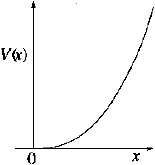
\includegraphics[width=0.2\columnwidth]{figs/35.png}
	\end{figure}


\begin{enumerate} \begin{multicols}{4}
	\item $\frac{31}{10}\hbar\omega$ \item $\frac{25}{10}\hbar\omega$ \item $\frac{13}{10}\hbar\omega$ \item $\frac{11}{10}\hbar\omega$
\end{multicols} \end{enumerate}

\item Match the typical spectra of stable molecules with the corresponding wave-number range
\hfill\brak{\text{GATE PH 2010}}

\begin{multicols}{2}
 \begin{enumerate}
  \item Electronic Spectra
  \item Rotational Spectra
  \item Molecular dissociation
 \end{enumerate}
\columnbreak
\begin{itemize}
 \item $10^6 cm^{-1}$ and above
 \item $10^5 - 10^6 cm^{-1}$
 \item $10^0 - 10^2 cm^{-1}$
\end{itemize}


\end{multicols}


\begin{enumerate}
	\begin{multicols}{2}
	 \item 1-ii, 2-i, 3-iii \item 1-ii, 2-iii, 3-i \item 1-iii, 2-ii, 3-i \item 1-i, 2-ii, 3-iii
	\end{multicols}
\end{enumerate}

\item Consider the operations $P:\vec{r}\rightarrow-\vec{r}$ (parity) and $T:t\rightarrow-t$ (time-reversal). For the electric and magnetic fields $\vec{E}$ and $\vec{B}$, which of the following set of transformations is correct?\hfill\brak{\text{GATE PH 2010}}

\begin{enumerate}
	\begin{multicols}{2}
	 \item $P:\vec{E}\rightarrow-\vec{E},\vec{B}\rightarrow\vec{B};\\ T:\vec{E}\rightarrow\vec{E},\vec{B}\rightarrow-\vec{B}$
	\item $P:\vec{E}\rightarrow\vec{E},\vec{B}\rightarrow-\vec{B};\\ T:\vec{E}\rightarrow\vec{E},\vec{B}\rightarrow\vec{B}$
	\item $P:\vec{E}\rightarrow-\vec{E},\vec{B}\rightarrow\vec{B};\\ T:\vec{E}\rightarrow-\vec{E},\vec{B}\rightarrow-\vec{B}$
	\item $P:\vec{E}\rightarrow\vec{E},\vec{B}\rightarrow-\vec{B};\\ T:\vec{E}\rightarrow-\vec{E},\vec{B}\rightarrow\vec{B}$
	\end{multicols}
\end{enumerate}

\item Two magnetic dipoles of magnitude m each are placed in a plane as shown. The energy of interaction is given by\hfill\brak{\text{GATE PH 2010}}
	\begin{figure}[H] \centering
		\caption*{} \label{fig:38} 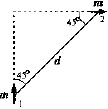
\includegraphics[width=0.1\columnwidth]{figs/38.png}
	\end{figure}


\begin{enumerate} \begin{multicols}{4}
	\item Zero \item $\frac{\mu_{0}}{4\pi}\frac{m^{2}}{d^{3}}$ \item $\frac{3\mu_{0}}{2\pi}\frac{m^{2}}{d^{3}}$ \item $-\frac{3\mu_{0}}{8\pi}\frac{m^{2}}{d^{3}}$
\end{multicols} \end{enumerate}

\item Consider a conducting loop of radius a and total loop resistance R placed in a region with a magnetic field B thereby enclosing a flux $\phi_0$. The loop is connected to an electronic circuit as shown, the capacitor being initially uncharged.
	\begin{figure}[H]
	\centering
		\caption*{} \label{fig:39} \caption*{} \label{fig:} 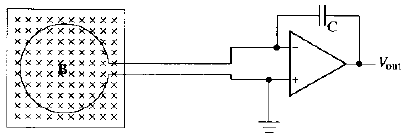
\includegraphics[width=0.8\columnwidth]{figs/39.png}
	\end{figure}
	If the loop is pulled out of the region of the magnetic field at a constant speed u, the final output voltage $V_{out}$ is independent of\hfill\brak{\text{GATE PH 2010}}


\begin{enumerate} \begin{multicols}{4}
	\item $\phi_0$ \item u \item R \item C
\end{multicols} \end{enumerate}

\item The figure shows a constant current source charging a capacitor that is initially uncharged.
	\begin{figure}[H] \centering
		\caption*{} \label{fig:40} 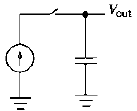
\includegraphics[width=0.3\columnwidth]{figs/40.png}
	\end{figure}
	If the switch is closed at $t=0$, which of the following plots depicts correctly the output voltage of the circuit as a function of time?\hfill\brak{\text{GATE PH 2010}}
	\begin{figure}[H]
		\centering
		\caption*{} \label{fig:40a} 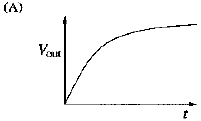
\includegraphics[width=0.45\columnwidth]{figs/40a.png}
		\caption*{} \label{fig:40b} 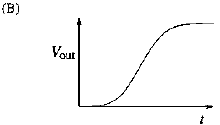
\includegraphics[width=0.45\columnwidth]{figs/40b.png}
		\caption*{} \label{fig:40c} 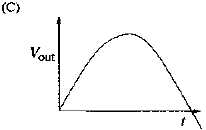
\includegraphics[width=0.45\columnwidth]{figs/40c.png}
		\caption*{} \label{fig:40d} 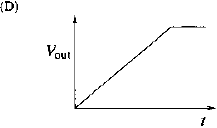
\includegraphics[width=0.45\columnwidth]{figs/40d.png}
	\end{figure}


\item For any set of inputs, A and B, the following circuits give the same output, Q, except one. Which one is it?\hfill\brak{\text{GATE PH 2010}}

\begin{enumerate} \begin{multicols}{2}
\begin{figure}[H]
	\item \caption*{} \label{fig:41a} 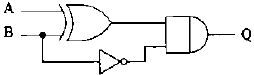
\includegraphics[width=0.51\columnwidth]{figs/41a.png}
	\item \caption*{} \label{fig:41b} 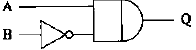
\includegraphics[width=0.51\columnwidth]{figs/41b.png}
	\item \caption*{} \label{fig:41c} 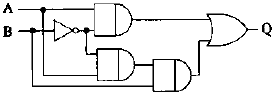
\includegraphics[width=0.51\columnwidth]{figs/41c.png}
	\item \caption*{} \label{fig:41d} 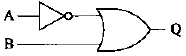
\includegraphics[width=0.51\columnwidth]{figs/41d.png}
\end{figure}
\end{multicols} \end{enumerate}

\item CO$_2$ molecule has the first few energy levels uniformly separated by approximately 2.5 meV. At a temperature of 300 K, the ratio of the number of molecules in the 4\textsuperscript{th} excited state to the number in the 2\textsuperscript{nd} excited state is about\hfill\brak{\text{GATE PH 2010}}

\begin{enumerate} \begin{multicols}{4}
	\item 0.5 \item 0.6 \item 0.8 \item 0.9
\end{multicols} \end{enumerate}

\item Which among the following sets of Maxwell relations is correct? (U- internal energy, H- enthalpy, A- Helmholtz free energy and G- Gibbs free energy)\hfill\brak{\text{GATE PH 2010}}

\begin{enumerate}
	\begin{multicols}{2}
	 \item $T = \left(\frac{\partial U}{\partial V}\right)_{S}$ and $P = -\left(\frac{\partial U}{\partial S}\right)_{V}$
	\item $V = \left(\frac{\partial H}{\partial P}\right)_{S}$ and $T = \left(\frac{\partial H}{\partial S}\right)_{P}$
	\item $P = -\left(\frac{\partial G}{\partial V}\right)_{T}$ and $V = -\left(\frac{\partial G}{\partial P}\right)_{S}$
	\item $P = -\left(\frac{\partial A}{\partial S}\right)_{T}$ and $S = -\left(\frac{\partial A}{\partial P}\right)_{V}$
	\end{multicols}
\end{enumerate}

\item For a spin-s particle, in the eigen basis of $\hat{S}^2,S$, the expectation value $\langle s m | S_x^2 | s m \rangle$ is\hfill\brak{\text{GATE PH 2010}}

\begin{enumerate}
	\begin{multicols}{2}
	 \item $\frac{\hbar^2[s(s+1)-m^2]}{2}$ \item $\hbar^2[s(s+1)-2m^2]$
	\item $\hbar^2[s(s+1)-m^2]$ \item $\hbar^2 m^2$
	\end{multicols}
\end{enumerate}

\item A particle is placed in a region with the potential $V(x)=\frac{1}{2}kx^2-\frac{1}{4}\lambda x^3$, where $k, \lambda > 0$. Then,\hfill\brak{\text{GATE PH 2010}}

\begin{enumerate}
	\item $x=0$ and $x=\pm\sqrt{\frac{k}{\lambda}}$ are points of stable equilibrium
	\item $x=0$ is a point of stable equilibrium and $x=\pm\sqrt{\frac{k}{\lambda}}$ is a point of unstable equilibrium
	\item $x=0$ and $x=\pm\sqrt{\frac{k}{\lambda}}$ are points of unstable equilibrium
	\item There are no points of stable or unstable equilibrium
\end{enumerate}

\item A $\pi^0$ meson at rest decays into two photons, which move along the x-axis. They are both detected simultaneously after a time, $t=10$ s. In an inertial frame moving with a velocity $V=0.6c$ in the direction of one of the photons, the time interval between the two detections is\hfill\brak{\text{GATE PH 2010}}

\begin{enumerate} \begin{multicols}{4}
	\item 15 s \item 0 s \item 10 s \item 20 s
\end{multicols} \end{enumerate}

\item A particle of mass m is confined in an infinite potential well: $$V(x) = \begin{cases} 0 & \text{if } 0<x<L, \\ \infty & \text{otherwise} \end{cases}$$. It is subjected to a perturbing potential $V_p(x) = V_0 \sin\left(\frac{2\pi x}{L}\right)$ within the well. Let $E^{(1)}$ and $E^{(2)}$ be the corrections to the ground state energy in the first and second order in $V_0$, respectively. Which of the following are true?\hfill\brak{\text{GATE PH 2010}}
	\begin{figure}[H] \centering
		\caption*{} \label{fig:47} 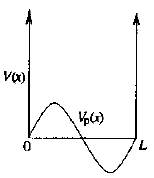
\includegraphics[width=0.4\columnwidth]{figs/47.png}
	\end{figure}


\begin{enumerate}
	\begin{multicols}{2}
	 \item $E^{(1)}=0; \quad E^{(2)}<0$ \item $E^{(1)}>0; \quad E^{(2)}=0$
	\item $E^{(1)}=0; \quad E^{(2)}$ depends on the sign of $V_0$ \item $E^{(1)}<0; \quad E^{(2)}<0$
	\end{multicols}
\end{enumerate}

\par\noindent In the presence of a weak magnetic field, atomic hydrogen undergoes the transition:
\begin{align*} ^2P_{3/2} \rightarrow ^2S_{1/2} \end{align*}
by emission of radiation.

\item The number of distinct spectral lines that are observed in the resultant Zeeman spectrum is\par\hfill\brak{\text{GATE PH 2010}}

\begin{enumerate} \begin{multicols}{4}
	\item 2 \item 3 \item 4 \item 6
\end{multicols} \end{enumerate}

\item The spectral line corresponding to the transition \begin{align*}^2P_{3/2} \left(m_j = +\frac{1}{2}\right) \rightarrow ^2S_{1/2} \left(m_j = -\frac{1}{2}\right)\end{align*} is observed along the direction of the applied magnetic field. The emitted electromagnetic field is:\hfill\brak{\text{GATE PH 2010}}

\begin{enumerate}
	\begin{multicols}{2}
	 \item Circularly polarized \item Linearly polarized \item Unpolarized \item Not emitted along the magnetic field direction
	\end{multicols}
\end{enumerate}

\textbf{Common Data for Questions 50 and 51:}
\par\noindent The partition function for a gas of photons is given by
\begin{align*} \ln Z = \frac{\pi^2 V(k_B T)^3}{45 \hbar^3 c^3} \end{align*}

\item The specific heat of the photon gas varies with temperature as\hfill\brak{\text{GATE PH 2010}}
\begin{figure}[H]
	\centering
	\caption*{} \label{fig:50a} 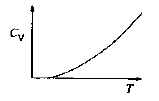
\includegraphics[width=0.35\columnwidth]{figs/50a.png}
	\caption*{} \label{fig:50b} 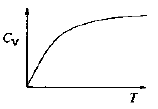
\includegraphics[width=0.35\columnwidth]{figs/50b.png}
	\caption*{} \label{fig:50c} 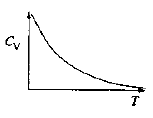
\includegraphics[width=0.35\columnwidth]{figs/50c.png}
	\caption*{} \label{fig:50d} 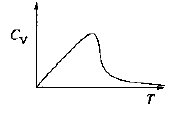
\includegraphics[width=0.35\columnwidth]{figs/50d.png}
\end{figure}

\item The pressure of the photon gas is\hfill\brak{\text{GATE PH 2010}}

\begin{enumerate} \begin{multicols}{4}
	\item $\frac{\pi^2(k_B T)^4}{15 \hbar^3 c^3}$ \item $\frac{\pi^2(k_B T)^4}{8 \hbar^3 c^3}$
	\item $\frac{\pi^2(k_B T)^4}{45 \hbar^3 c^3}$ \item $\frac{\pi(k_B T)^4}{45 \hbar^3 c^3}$
\end{multicols} \end{enumerate}

\par\noindent Consider the propagation of electromagnetic waves in a linear, homogeneous and isotropic material medium with electric permittivity $\epsilon$ and magnetic permeability $\mu$.

\item For a plane wave of angular frequency $\omega$ and propagation vector $\vec{k}$ propagating in the medium Maxwell's equations reduce to\hfill\brak{\text{GATE PH 2010}}

\begin{enumerate}
	\item $\vec{k} \cdot \vec{E} = 0; \quad \vec{k} \cdot \vec{H} = 0; \quad \vec{k} \times \vec{E} = \omega\epsilon\vec{H}; \quad \vec{k} \times \vec{H} = -\omega\mu\vec{E}$
	\item $\vec{k} \cdot \vec{E} = 0; \quad \vec{k} \cdot \vec{H} = 0; \quad \vec{k} \times \vec{E} = -\omega\epsilon\vec{H}; \quad \vec{k} \times \vec{H} = \omega\mu\vec{E}$
	\item $\vec{k} \cdot \vec{E} = 0; \quad \vec{k} \cdot \vec{H} = 0; \quad \vec{k} \times \vec{E} = -\omega\mu\vec{H}; \quad \vec{k} \times \vec{H} = \omega\epsilon\vec{E}$
	\item $\vec{k} \cdot \vec{E} = 0; \quad \vec{k} \cdot \vec{H} = 0; \quad \vec{k} \times \vec{E} = \omega\mu\vec{H}; \quad \vec{k} \times \vec{H} = -\omega\epsilon\vec{E}$
\end{enumerate}

\item If $\epsilon$ and $\mu$ assume negative values in a certain frequency range, then the directions of the propagation vector $\vec{k}$ and the Poynting vector $\vec{S}$ in that frequency range are related as\hfill\brak{\text{GATE PH 2010}}

\begin{enumerate}
	\item $\vec{k}$ and $\vec{S}$ are parallel \item $\vec{k}$ and $\vec{S}$ are anti-parallel
	\item $\vec{k}$ and $\vec{S}$ are perpendicular to each other
	\item $\vec{k}$ and $\vec{S}$ make an angle that depends on the magnitude of $|\epsilon|$ and $|\mu|$
\end{enumerate}

\par\noindent The Lagrangian for a simple pendulum is given by:
\begin{align*} L = \frac{1}{2}ml^2\dot{\theta}^2 - mgl(1-\cos\theta) \end{align*}

\item Hamilton's equations are then given by\hfill\brak{\text{GATE PH 2010}}

\begin{enumerate}
	\begin{multicols}{2}
	 \item $p_{\theta} = -mgl\sin\theta; \quad \dot{\theta} = \frac{p_{\theta}}{ml^2}$
	\item $p_{\theta} = mgl\sin\theta; \quad \dot{\theta} = \frac{p_{\theta}}{ml^2}$
	\item $p_{\theta} = -m\ddot{\theta}; \quad \dot{\theta} = \frac{p_{\theta}}{m}$
	\item $\dot{p_{\theta}} = -\left(\frac{g}{l}\right)\theta; \quad \dot{\theta} = \frac{p_{\theta}}{ml}$
	\end{multicols}
\end{enumerate}

\item The Poisson bracket between $\theta$ and $\dot{\theta}$ is\hfill\brak{\text{GATE PH 2010}}

\begin{enumerate} \begin{multicols}{4}
	\item $\{\theta, \dot{\theta}\} = 1$ \item $\{\theta, \dot{\theta}\} = \frac{1}{ml^2}$
	\item $\{\theta, \dot{\theta}\} = \frac{1}{m}$ \item $\{\theta, \dot{\theta}\} = \frac{g}{l}$
\end{multicols} \end{enumerate}
\newpage

\item \textit{Choose the most appropriate word from the options given below to complete the following sentence.}\hfill\brak{\text{GATE PH 2010}}\par
	\textbf{\noindent His rather casual remarks on politics \rule{2cm}{0.4pt} his lack of seriousness about the subject.}

\begin{enumerate} \begin{multicols}{4}
	\item masked \item belied \item betrayed \item suppressed
\end{multicols} \end{enumerate}

\item Which of the following options is the closest in meaning to the word below:\hfill\brak{\text{GATE PH 2010}}\par\noindent \textbf{Circuitous}

\begin{enumerate} \begin{multicols}{4}
	\item cyclic \item indirect \item confusing \item crooked
\end{multicols} \end{enumerate}

\item \textit{Choose the most appropriate word from the options given below to complete the following sentence:}\hfill\brak{\text{GATE PH 2010}}
	\par\noindent \textbf{If we manage to \rule{2cm}{0.4pt} our natural resources, we would leave a better planet for our children.}

\begin{enumerate} \begin{multicols}{4}
	\item uphold \item restrain \item cherish \item conserve
\end{multicols} \end{enumerate}

\item 25 persons are in a room. 15 of them play hockey, 17 of them play football and 10 of them play both hockey and football. Then the number of persons playing neither hockey nor football is:\hfill\brak{\text{GATE PH 2010}}

\begin{enumerate} \begin{multicols}{4}
	\item 2 \item 17 \item 13 \item 3
\end{multicols} \end{enumerate}

\item \textit{The question below consists of a pair of related words followed by four pairs of words. Select the pair that best expresses the relation in the original pair.}\hfill\brak{\text{GATE PH 2010}}
	\par\noindent\textbf{Unemployed : Worker}

\begin{enumerate} \begin{multicols}{4}
	\item fallow : land \item unaware : sleeper \item wit : jester \item renovated : house
\end{multicols} \end{enumerate}

\item If $137 + 276 = 435$ how much is $731 + 672$?\hfill\brak{\text{GATE PH 2010}}

\begin{enumerate} \begin{multicols}{4}
	\item 534 \item 1403 \item 1623 \item 1513
\end{multicols} \end{enumerate}

\item Hari (H), Gita (G), Irfan (I) and Saira (S) are siblings (i.e. brothers and sisters). All were born on 1\textsuperscript{st} January. The age difference between any two successive siblings (that is born one after another) is less than 3 years. Given the following facts:

\begin{enumerate}
		\item Hari's age + Gita's age $>$ Irfan's age + Saira's age.
		\item The age difference between Gita and Saira is 1 year. However, Gita is not the oldest and Saira is not the youngest.
		\item There are no twins.
	\end{enumerate}
	In what order were they born (oldest first)?\hfill\brak{\text{GATE PH 2010}}


\begin{enumerate} \begin{multicols}{4}
	\item HSIG \item SGHI \item IGSH \item IHSG
\end{multicols} \end{enumerate}

\item \textbf{Modern warfare has changed from large scale clashes of armies to suppression of civilian populations. Chemical agents that do their work silently appear to be suited to such warfare; and regretfully, there are people in military establishments who think that chemical agents are useful tools for their cause.}
	\par\noindent \textit{Which of the following statements best sums up the meaning of the above passage:}\hfill\brak{\text{GATE PH 2010}}

\begin{enumerate}
	\item Modern warfare has resulted in civil strife.
	\item Chemical agents are useful in modern warfare.
	\item Use of chemical agents in warfare would be undesirable.
	\item People in military establishments like to use chemical agents in war.
\end{enumerate}

\item 5 skilled workers can build a wall in 20 days; 8 semi-skilled workers can build a wall in 25 days; 10 unskilled workers can build a wall in 30 days. If a team has 2 skilled, 6 semi-skilled and 5 unskilled workers, how long will it take to build the wall?\hfill\brak{\text{GATE PH 2010}}

\begin{enumerate} \begin{multicols}{4}
	\item 20 days \item 18 days \item 16 days \item 15 days
\end{multicols} \end{enumerate}

\item Given digits 2, 2, 3, 3, 3, 4, 4, 4, 4 how many distinct 4 digit numbers greater than 3000 can be formed?\hfill\brak{\text{GATE PH 2010}}

\begin{enumerate} \begin{multicols}{4}
	\item 50 \item 51 \item 52 \item 54
\end{multicols} \end{enumerate}
\end{enumerate}

\hrulefill
\begin{center}
\begin{tabular}{c}
\textbf{END OF THE QUESTION PAPER}
\end{tabular}
\end{center}

\end{document}
